\section{Layer Demand Is Heterogeneous}
\label{sec:heterogeneity}

\begin{figure}[t]
    \centering
    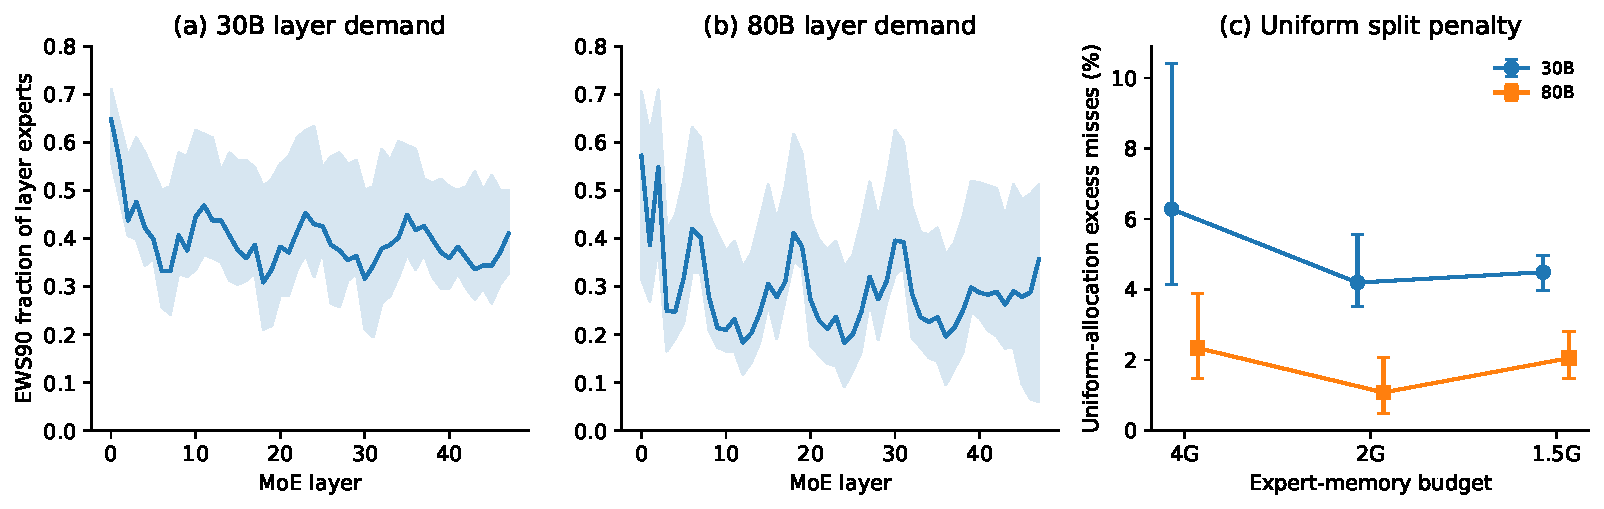
\includegraphics[width=\linewidth]{../experiments/EXP-007-router-characterization/figures/layer_heterogeneity_and_uniform_penalty.pdf}
    \caption{Layer demand is heterogeneous and uniform memory partitioning is measurably suboptimal. Panels (a) and (b) show the median per-layer EWS90 fraction across the 14 final in-sample workload/split cells for the 30B and 80B MoEs; shaded regions denote the full observed range. Layer-demand heterogeneity is present in both models, with per-cell EWS90 coefficients of variation spanning 0.085--0.248 for 30B and 0.162--0.455 for 80B. Panel (c) shows the median excess misses induced by a uniform per-layer memory split, with whiskers denoting the full observed range. The result establishes measurable allocation opportunity but does not imply that greater routing heterogeneity necessarily yields greater allocation benefit.}
    \label{fig:heterogeneity}
\end{figure}
